\documentclass[11pt,a4paper]{article}
\newcommand{\simname}{Shot Peening Coverage Simulator}
\usepackage[utf8]{inputenc}
\usepackage[T1]{fontenc}
\usepackage[sc]{mathpazo}
\linespread{1.05}
\usepackage[english]{babel}
\usepackage[margin=2.2cm]{geometry}
\usepackage{amsmath,amssymb}
\usepackage[locale=UK,per-mode=symbol]{siunitx}
\usepackage{booktabs,array,tabularx,longtable}
\usepackage{graphicx}
\usepackage{tikz}
\usetikzlibrary{arrows.meta,decorations.pathreplacing,calc}
\usepackage{xcolor}
\usepackage[hidelinks]{hyperref}
\usepackage{enumitem}
\usepackage{tcolorbox}
\usepackage{float}
\usepackage[font=small,labelfont=bf]{caption}
\usepackage{subcaption}
\usepackage{fancyhdr}
\usepackage{multicol}

\definecolor{bleu}{HTML}{1F5A96}
\definecolor{orange}{HTML}{D4621C}
\definecolor{vert}{HTML}{2E8B57}
\definecolor{rouge}{HTML}{E5484D}
\newtcolorbox{keybox}[1][]{colback=bleu!5,colframe=bleu,boxrule=0.6pt,arc=2pt,left=6pt,right=6pt,top=4pt,bottom=4pt,#1}
\newtcolorbox{trybox}[1][]{colback=orange!6,colframe=orange,boxrule=0.6pt,arc=2pt,left=6pt,right=6pt,top=4pt,bottom=4pt,#1}
\newcommand{\E}{\mathbb{E}}
\newcommand{\dX}{\Delta X}
\newcommand{\ui}[1]{\textsf{#1}}   % name of a control or a readout on the page
\setlength{\tabcolsep}{5pt}
\renewcommand{\arraystretch}{1.15}

\pagestyle{fancy}
\fancyhf{}
\fancyhead[L]{\small Dr Régis Kubler, Arts et Métiers Institute of Technology}
\fancyhead[R]{\small\simname}
\fancyfoot[C]{\small\thepage}
\renewcommand{\headrulewidth}{0.4pt}
\setlength{\headheight}{14pt}
\setlength{\parskip}{3pt}
\usepackage{newunicodechar}
\newunicodechar{λ}{\ensuremath{\lambda}}
\newunicodechar{Σ}{\ensuremath{\Sigma}}
\newunicodechar{Δ}{\ensuremath{\Delta}}
\newunicodechar{δ}{\ensuremath{\delta}}
\newunicodechar{τ}{\ensuremath{\tau}}
\newunicodechar{σ}{\ensuremath{\sigma}}
\newunicodechar{η}{\ensuremath{\eta}}
\newunicodechar{α}{\ensuremath{\alpha}}
\newunicodechar{φ}{\ensuremath{\varphi}}
\newunicodechar{ζ}{\ensuremath{\zeta}}
\newunicodechar{²}{\ensuremath{^2}}
\newunicodechar{³}{\ensuremath{^3}}
\newunicodechar{−}{\ensuremath{-}}
\newunicodechar{·}{\ensuremath{\cdot}}
\newunicodechar{×}{\ensuremath{\times}}
\newunicodechar{≈}{\ensuremath{\approx}}
\newunicodechar{≥}{\ensuremath{\geq}}
\newunicodechar{≤}{\ensuremath{\leq}}
\newunicodechar{→}{\ensuremath{\rightarrow}}
\newunicodechar{°}{\ensuremath{^\circ}}
\newunicodechar{µ}{\ensuremath{\mu}}
\newunicodechar{…}{\ldots}
\newunicodechar{ṁ}{\ensuremath{\dot m}}
\newunicodechar{Ṅ}{\ensuremath{\dot N}}
\newunicodechar{₀}{\ensuremath{_0}}
\newunicodechar{₉}{\ensuremath{_9}}
\newunicodechar{₈}{\ensuremath{_8}}
\newunicodechar{₅}{\ensuremath{_5}}


\title{\textbf{Shot Peening Coverage Simulator}\\[3pt]
\large User and theory guide: local coverage under the jet}
\author{Dr Régis Kubler\\ Arts et Métiers Institute of Technology\\[4pt]
\small Developed with the assistance of Claude Opus 5.5 (Anthropic), November 2026}
\date{Guide for simulator version 1.5 (18 November 2026)\\ \url{https://rkubler.github.io/peening-coverage/}}

\begin{document}
\maketitle
\thispagestyle{fancy}

\begin{abstract}
\noindent This guide explains the Shot Peening Coverage Simulator, a web page that shows how the surface of a part becomes covered with dents during shot peening. It starts with the basic idea and a first experiment, then explains every equation, every parameter, every number and every chart displayed on the page, and finally the specified coverages above 100\,\% (treatment times) defined by NF~L~06-832. No installation is needed: the page runs in any web browser.
\end{abstract}

\tableofcontents

\section{The idea in one page}

\paragraph{What is coverage?} When a shot hits a metal surface it leaves a small round dent. The \emph{coverage} $\tau$ is the share of the surface that carries at least one dent. A fresh surface has $\tau=0$; a fully dented surface has $\tau=100\,\%$.

\paragraph{Why does it never quite reach 100\,\%?} Shots land at random. After a while most new shots fall on places that are already dented, and the last untouched spots are hit only by chance. Coverage therefore grows quickly at first, then more and more slowly. The law is
\begin{equation}
\boxed{\tau(n)=100\,\bigl(1-e^{-K n}\bigr)}
\label{eq:main}
\end{equation}
where $n$ is the number of passes of the jet and $K$ is the dented area brought by one pass, counted as if dents never overlapped. Everything on the page revolves around this formula and around the value of $K$.

\paragraph{What the page shows.} A nozzle sweeps a square part line by line at speed $V$ with a jet of width $\dX$ (Fig.~\ref{fig:sweep}). A small square of about half a millimetre in the middle of the part is observed under a ``microscope''. Each shot that lands in it draws a dent; the page counts the points that have been hit and compares the result with Eq.~\eqref{eq:main}.

\begin{figure}[H]
\centering
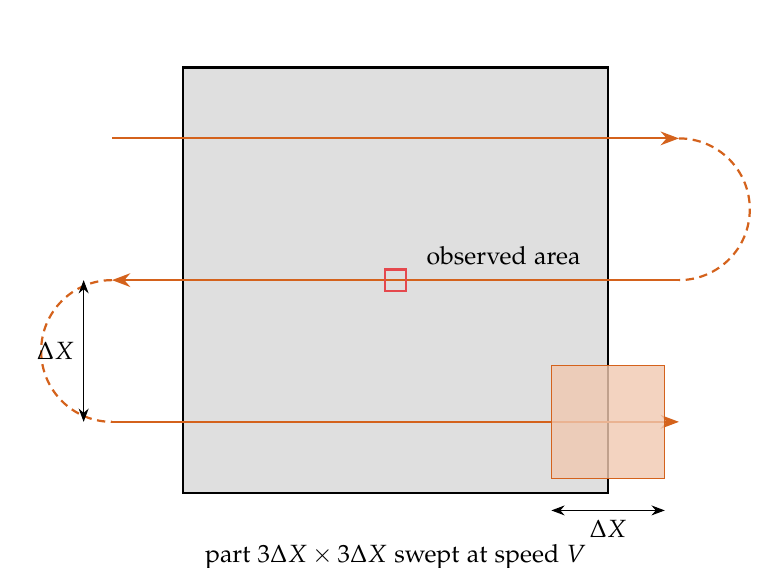
\begin{tikzpicture}[scale=0.9,>=Stealth]
\fill[gray!25] (0,0) rectangle (6,6); \draw[thick] (0,0) rectangle (6,6);
\foreach \y/\d in {5/1,3/-1,1/1}{ \ifnum\d=1 \draw[orange,thick,->] (-1,\y) -- (7,\y); \else \draw[orange,thick,->] (7,\y) -- (-1,\y); \fi }
\draw[orange,thick,densely dashed] (7,5) arc (90:-90:1); \draw[orange,thick,densely dashed] (-1,3) arc (90:270:1);
\fill[orange!35,opacity=.8] (5.2,0.2) rectangle (6.8,1.8); \draw[orange] (5.2,0.2) rectangle (6.8,1.8);
\draw[<->] (5.2,-0.25) -- (6.8,-0.25) node[midway,below] {\small $\dX$};
\draw[rouge,thick] (2.85,2.85) rectangle (3.15,3.15); \node[font=\small,anchor=west] at (3.3,3.35) {observed area};
\draw[<->] (-1.4,1) -- (-1.4,3) node[midway,left] {\small $\dX$};
\node[font=\small] at (3,-0.9) {part $3\dX\times3\dX$ swept at speed $V$};
\end{tikzpicture}
\caption{The jet sweeps the part along three lines spaced by $\dX$; the observed area sits on the middle line. Each point is under the jet once per pass.}
\label{fig:sweep}
\end{figure}

\begin{trybox}
\textbf{First experiment.} Open the page: it plays by itself with the reference values of the Excel model ($\dot m=\SI{1.5}{kg/min}$, glass beads $\rho=\SI{2.2}{g/cm^3}$, $D=\SI{150}{\micro m}$, dents $r=\SI{10}{\micro m}$, $\dX=\SI{20}{mm}$, $V=\SI{300}{mm/s}$). You get $K=0.337$, so:
\begin{itemize}[nosep]
\item after 1 pass, $\tau=1-e^{-0.337}=\SI{28.6}{\percent}$ of the surface is dented;
\item 98\,\% is reached after $n_{98}=\ln 50/K=11.6$ passes;
\item full coverage in the sense of NF~L~06-832 (1.25 times that time) needs $14.5$ passes.
\end{itemize}
Click \ui{Run all}: after 15 passes the measured coverage is about \SI{99.3}{\percent}, the model gives \SI{99.4}{\percent}. Click \ui{Restart} and run again: the dents fall elsewhere and the measured values change slightly, because the process is random.
\end{trybox}

\section{The screen}

\begin{figure}[H]
\centering
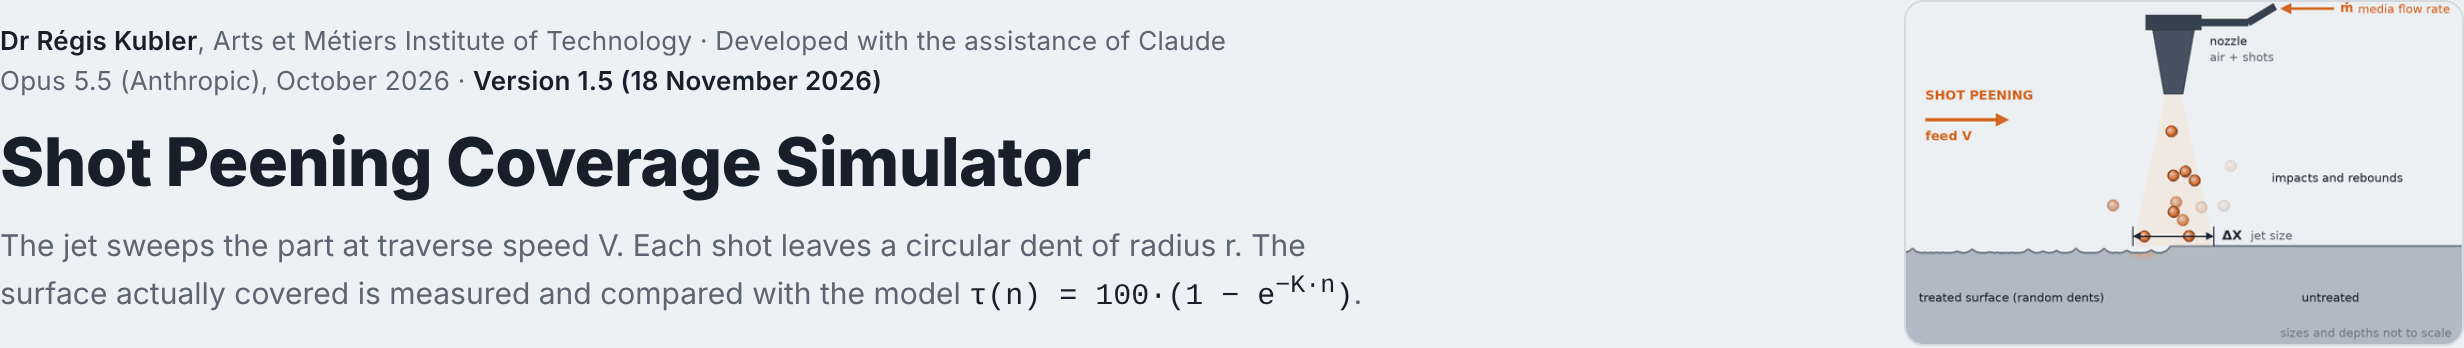
\includegraphics[width=\linewidth]{img/header.png}\\[2pt]

\includegraphics[width=\linewidth]{img/toolbar.png}
\caption{Title and toolbar of the page.}
\end{figure}

\paragraph{Toolbar.}
\begin{description}[leftmargin=2.6cm,style=nextline,itemsep=2pt]
\item[\ui{Play / Pause}] runs or stops the animation; at the end it becomes \ui{Replay}.
\item[\ui{+1 pass}] plays exactly one more pass and stops.
\item[\ui{Run all}] computes all the passes at once (no animation).
\item[\ui{Restart}] clears the part and draws a new random sequence of shots.
\item[\ui{Animation speed}] $\times0.5$ to $\times4$. It changes only the speed of the drawing, not the physics.
\item[\ui{Fast-forward outside the zone}] skips quickly over the parts of the path where the jet is far from the observed area.
\item[\ui{Show unimpacted surface}] paints in red the points that have not been hit yet. This makes the last gaps easy to see.
\end{description}

\paragraph{Panels.} The page is organised in six panels:
\begin{enumerate}[nosep]
\item \textbf{Observed area, microscope view}: the dents, coloured by the pass that made them, and the main readouts (Section~\ref{sec:reads}).
\item \textbf{Jet sweeping the part}: the path of the jet and the chart of coverage versus the number of passes (Section~\ref{sec:chart}).
\item \textbf{Map: how many times each point was hit}, with a slider to replay the map after any pass.
\item \textbf{Distribution: share of the surface hit $k$ times}, compared with the Poisson law.
\item \textbf{Parameters}, coverage above 100\,\% and the shot size distribution.
\item \textbf{How coverage is calculated}: the calculation chain, step by step, with the current values.
\end{enumerate}

\begin{figure}[H]
\centering
\begin{subfigure}{0.49\linewidth}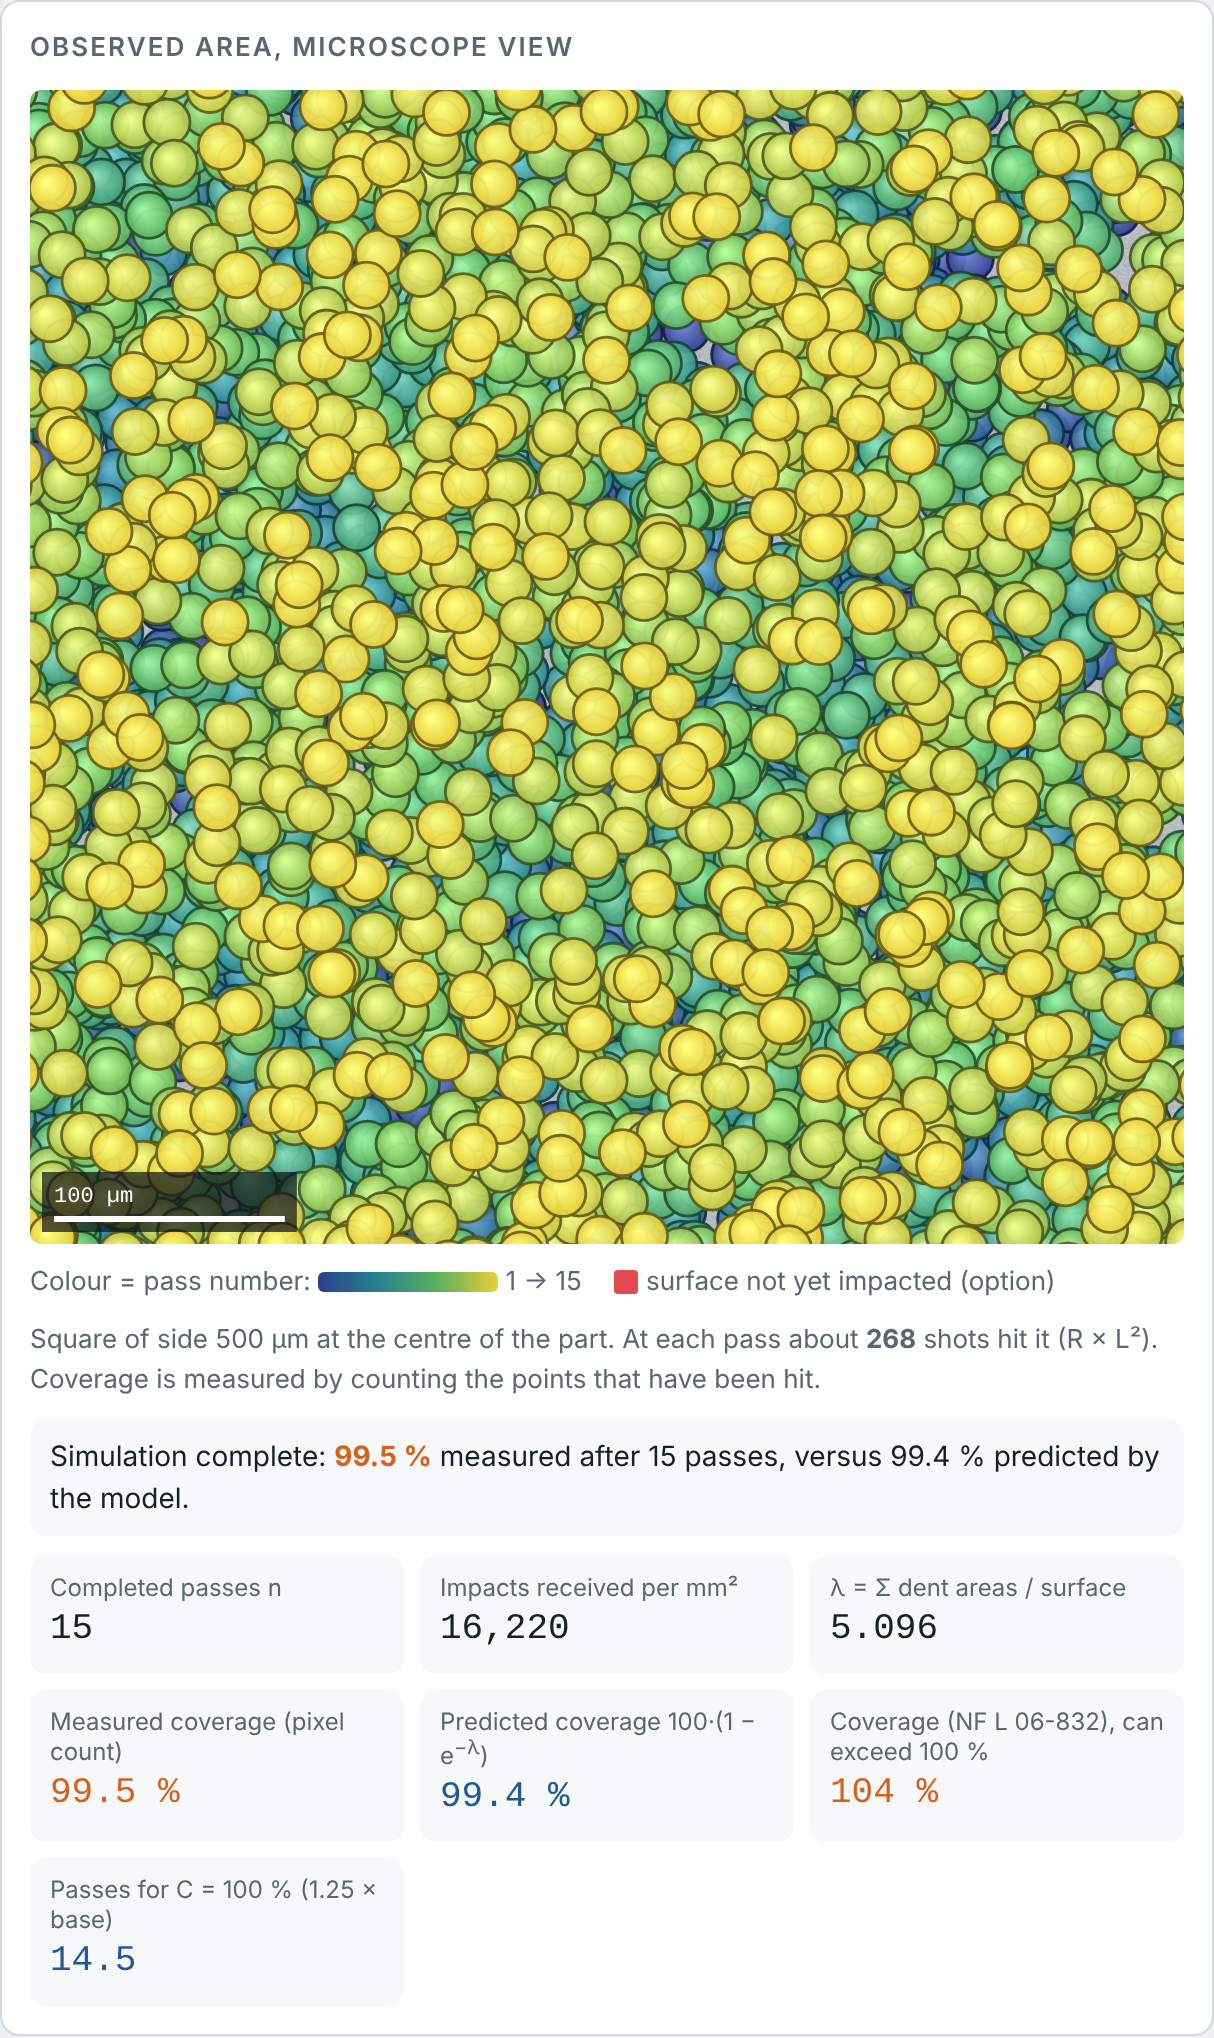
\includegraphics[width=\linewidth]{img/sec0.png}\caption{Microscope view and readouts}\end{subfigure}\hfill
\begin{subfigure}{0.49\linewidth}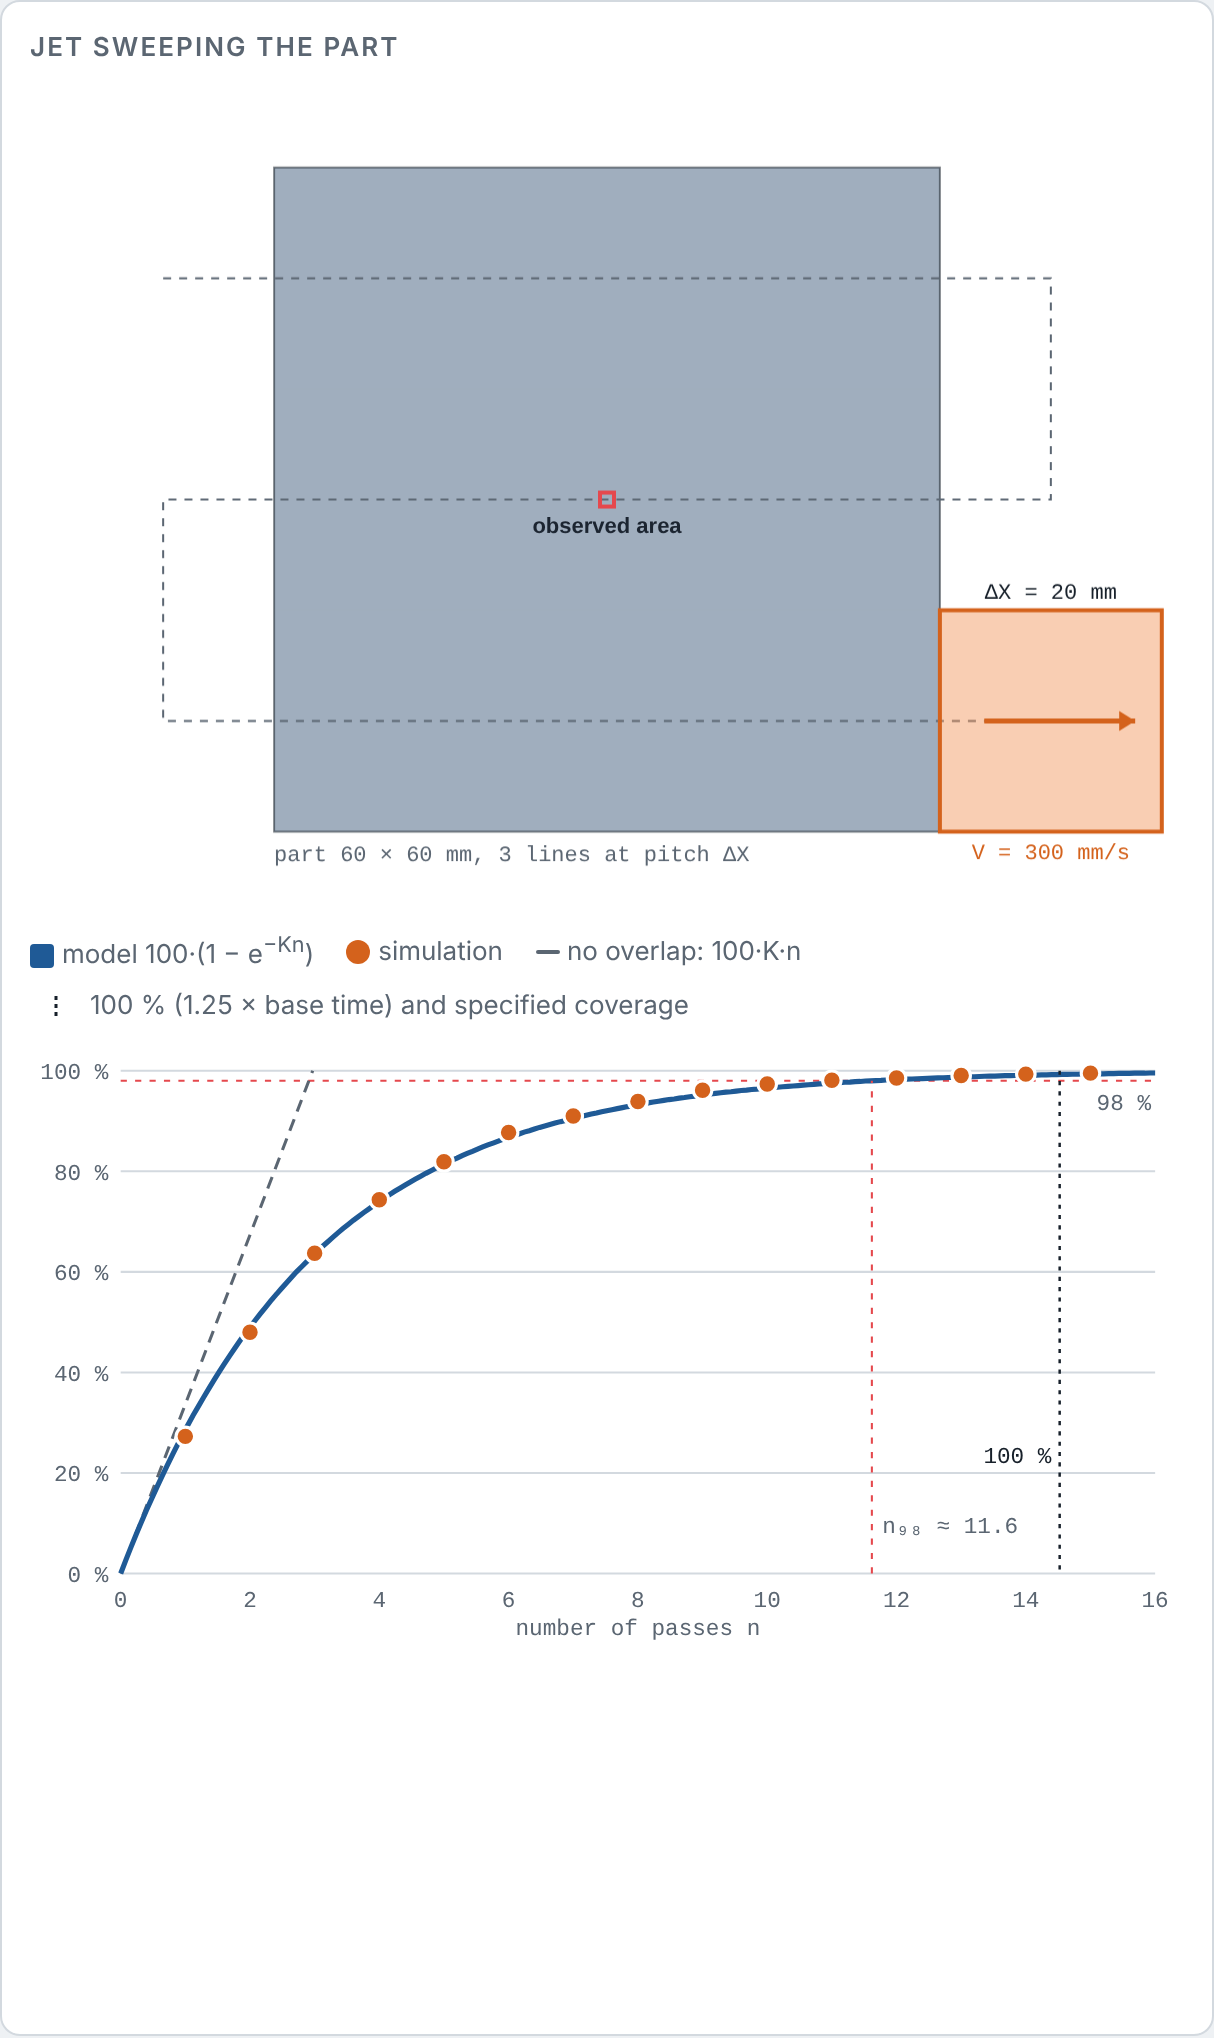
\includegraphics[width=\linewidth]{img/sec1.png}\caption{Sweep and coverage chart}\end{subfigure}
\caption{The two upper panels after 15 passes with the reference values.}
\end{figure}

\section{The model step by step}\label{sec:model}

The calculation chain at the bottom of the page follows these steps. The values in brackets are those of the reference case.

\subsection{Mass of a shot and shots per second}
A shot of diameter $D$ and density $\rho$ has the mass $\rho\pi D^3/6$. Real media contain several sizes, so the page uses the mean of $D^3$ over all the shots, written $\E[D^3]$:
\begin{equation}
m_p=\rho\,\frac{\pi}{6}\,\E[D^3]\quad[\SI{3.89}{\micro g}],\qquad
\dot N=\frac{\dot m}{m_p}\quad[\num{6.43e6}\ \text{shots/s}].
\end{equation}
For identical shots $\E[D^3]=D^3$. Large shots weigh much more than small ones, so $\E[D^3]$ is larger than the cube of the mean diameter (Section~\ref{sec:sizes}).

\subsection{Impacts per square millimetre in one pass}
The jet moves at speed $V$ and has the width $\dX$: it sweeps the area $V\dX$ every second. The number of shots that land on one square millimetre during one pass is
\begin{equation}
R=\frac{\dot N}{V\,\dX}\quad[\SI{1072}{/mm^2}].
\end{equation}
A point stays under the jet during the \emph{dwell time} $\dX/V$ [\SI{67}{ms}]. The jet is taken as uniform over its width.

\subsection{Area fraction dented per pass: the constant $K$}
Each impact leaves a dent of radius $r$, area $\pi r^2$. Adding up the dents of one pass, without removing overlaps,
\begin{equation}
K=\pi\,\E[r^2]\,R\quad[0.337].
\label{eq:K}
\end{equation}
$K$ is ``the fraction of the surface that one pass would dent if dents never overlapped''. With dents proportional to the shot, $r=c\,D$ where $c=r_{50}/D_{50}$ is the ratio entered on the page, $K$ can also be written
\begin{equation}
K=\frac{6\,\dot m\,c^2}{\rho\,D_{32}\,V\,\dX},\qquad D_{32}=\frac{\E[D^3]}{\E[D^2]},
\label{eq:Kalt}
\end{equation}
with $\dot m$ in kg/s and lengths in metres. This form shows how each parameter acts: $K$ doubles if the flow rate doubles or if the dent radius grows by $\sqrt2$; it halves if the speed or the jet size doubles.

\subsection{Random impacts: the Poisson law}
After $n$ passes a point has received on average $\lambda=K\,n$ impacts. Because shots land at random and independently, the number of impacts $k$ at a point follows the Poisson law
\begin{equation}
P(k)=e^{-\lambda}\,\frac{\lambda^k}{k!}.
\label{eq:poisson}
\end{equation}
The untouched surface is $P(0)=e^{-\lambda}$, hence Eq.~\eqref{eq:main}: $\tau=1-e^{-Kn}$. Two numbers follow:
\begin{equation}
n_{98}=\frac{\ln 50}{K}\ [11.6],\qquad \lambda_{98}=\ln 50=3.91.
\end{equation}
At 98\,\% coverage a point has received about four impacts on average, and some points many more.

\subsection{The no-overlap line}
If dents never overlapped, coverage would grow linearly, $100\,K\,n$, and reach 100\,\% after $1/K$ passes (3 passes here). The grey dashed line of the chart shows this; the gap between it and the curve is the effect of overlap.

\section{Shot size distribution}\label{sec:sizes}

With $\sigma=0$ all shots have the diameter $D_{50}$: this reproduces the reference Excel model. With $\sigma>0$ the diameters follow a log-normal law. Sieving gives the distribution \emph{by mass}, so $D_{50}$ is the mass median diameter. The page derives:
\begin{align}
D_{50,\text{number}}&=D_{50}\,e^{-3\sigma^2}, &
\E[D^3]&=D_{50}^3\,e^{-4.5\sigma^2}, &
\E[D^2]&=D_{50}^2\,e^{-4\sigma^2}, &
D_{32}&=D_{50}\,e^{-\sigma^2/2}.
\end{align}
The size chart of the parameter panel draws the distribution by number (blue) and by mass (orange), with markers at $D_{50}$ (mass), $D_{32}$ and $D_{50}$ (number). The note below the chart gives the range of dent radii (95\,\% of the shots) and compares $K$ with the value for identical shots. The single-size model stays exact if $D_{32}$ is used instead of $D_{50}$ (Eq.~\ref{eq:Kalt}).

\begin{keybox}
\textbf{Example.} With $\sigma=0.3$ and the other reference values: $D_{32}=\SI{143}{\micro m}$, the mean shot is lighter ($m_p=\SI{2.59}{\micro g}$), more shots are thrown ($\num{9.64e6}$/s), and $K$ rises from 0.337 to 0.352: 98\,\% is reached in 11.1 passes instead of 11.6.
\end{keybox}

\section{How the page simulates the shots}\label{sec:sim}

\begin{enumerate}[leftmargin=*]
\item \textbf{Observed area.} A square of side $L=50\,r_{\text{rms}}$ [\SI{500}{\micro m}], reduced if needed so that a pass never holds more than about 2\,500 shots. Shots are drawn on a slightly larger square (by the largest dent radius on each side), so that dents straddling the edges are included.
\item \textbf{Number of shots per pass.} Drawn from a Poisson law of mean $R\times(\text{sampling area})$ [about 290]; about 268 of them land inside the observed square (shown under the microscope view).
\item \textbf{Each shot.} A uniform random position, a log-normal random diameter (Box--Muller method), and a dent radius $r=cD$.
\item \textbf{Timing.} During the animation the dents of a pass appear while the jet crosses the observed area.
\item \textbf{Measurement.} The observed square carries a grid of $500\times500$ points. Each dent adds 1 to every grid point inside its circle. The measured coverage is the share of points with at least one hit; the map and the histogram use the same counts.
\end{enumerate}
Because the shots are random, two runs never give exactly the same numbers. The scatter is about one percent here, since the area holds only a few hundred dents per pass.

\section{Every result displayed}\label{sec:reads}

\begin{longtable}{@{}p{4.3cm}p{6.6cm}p{2.6cm}@{}}
\toprule
\textbf{Readout} & \textbf{Meaning and formula} & \textbf{Reference case}\\ \midrule\endhead
\ui{Completed passes n} & passes done so far & 15\\
\ui{Impacts received per mm²} & shots that landed in the observed square, divided by its area & about \num{16100}\\
\ui{λ = Σ dent areas / surface} & sum of the areas of the dents drawn, divided by the sampling area: the measured $K n$ & 5.06\\
\ui{Measured coverage (pixel count)} & share of grid points hit at least once & 99.3\,\%\\
\ui{Predicted coverage 100·(1 − e\textsuperscript{−λ})} & Eq.~\eqref{eq:main} with the measured $\lambda$ & 99.4\,\%\\
\ui{Coverage (NF L 06-832)} & dented area up to $t_b$, then time-based (Section~\ref{sec:above}) & $\approx$103\,\%\\
\ui{Passes for C = …} & inverse of $C(t)$; $\frac{C}{100}\times1.25\,\frac{\ln 50}{K}$ above 100\,\% & 14.5\\
\ui{Mean impacts per point} & mean of the hit-count map & 5.05\\
\ui{Predicted: λ = K·n} & theory for the mean & 5.05\\
\ui{Most-hit point} & maximum of the hit-count map & about 16\\
\ui{Never-hit surface (k = 0)} & share of points with no hit; theory $e^{-Kn}$ & 0.7\,\%\\
\bottomrule
\end{longtable}

\noindent The calculation chain repeats the intermediate values: mean shot mass $m_p$, shots per second $\dot N$, impacts per mm² per pass $R$ (with the dwell time $\dX/V$), $K$ (with $D_{32}$), $n_{98}$ and $n_{100}$. The step being animated is highlighted.

\section{Charts and maps}\label{sec:chart}

\paragraph{Coverage versus number of passes.} Blue curve: model $100(1-e^{-Kn})$. Orange dots: measured coverage after each pass. Grey dashed line: no-overlap growth $100Kn$. Red dotted line: 98\,\% level, with the marker $n_{98}$. Black dotted lines: 100\,\% coverage (1.25 times the base time) and the specified coverage $C$ when it differs from 100\,\%. The horizontal axis extends automatically to show these markers.

\paragraph{Hit-count map.} Each point of the observed area is coloured by the number of impacts it received: red for none, then light to dark blue up to 25 and more. During the animation the map follows the current pass; at the end the slider \ui{Map after} replays the map after any pass. Hovering gives the count at a point.

\paragraph{Distribution of hits.} Orange bars: share of the surface hit $k$ times (from the map). Blue dots: Poisson law~\eqref{eq:poisson} with $\lambda=Kn$. The bar at $k=0$ is the uncovered surface; the others show how unevenly the surface is peened. At 98\,\% coverage the mean is about 3.9 hits per point, at full coverage (100\,\%) about 4.9.

\begin{figure}[H]
\centering
\begin{subfigure}{0.49\linewidth}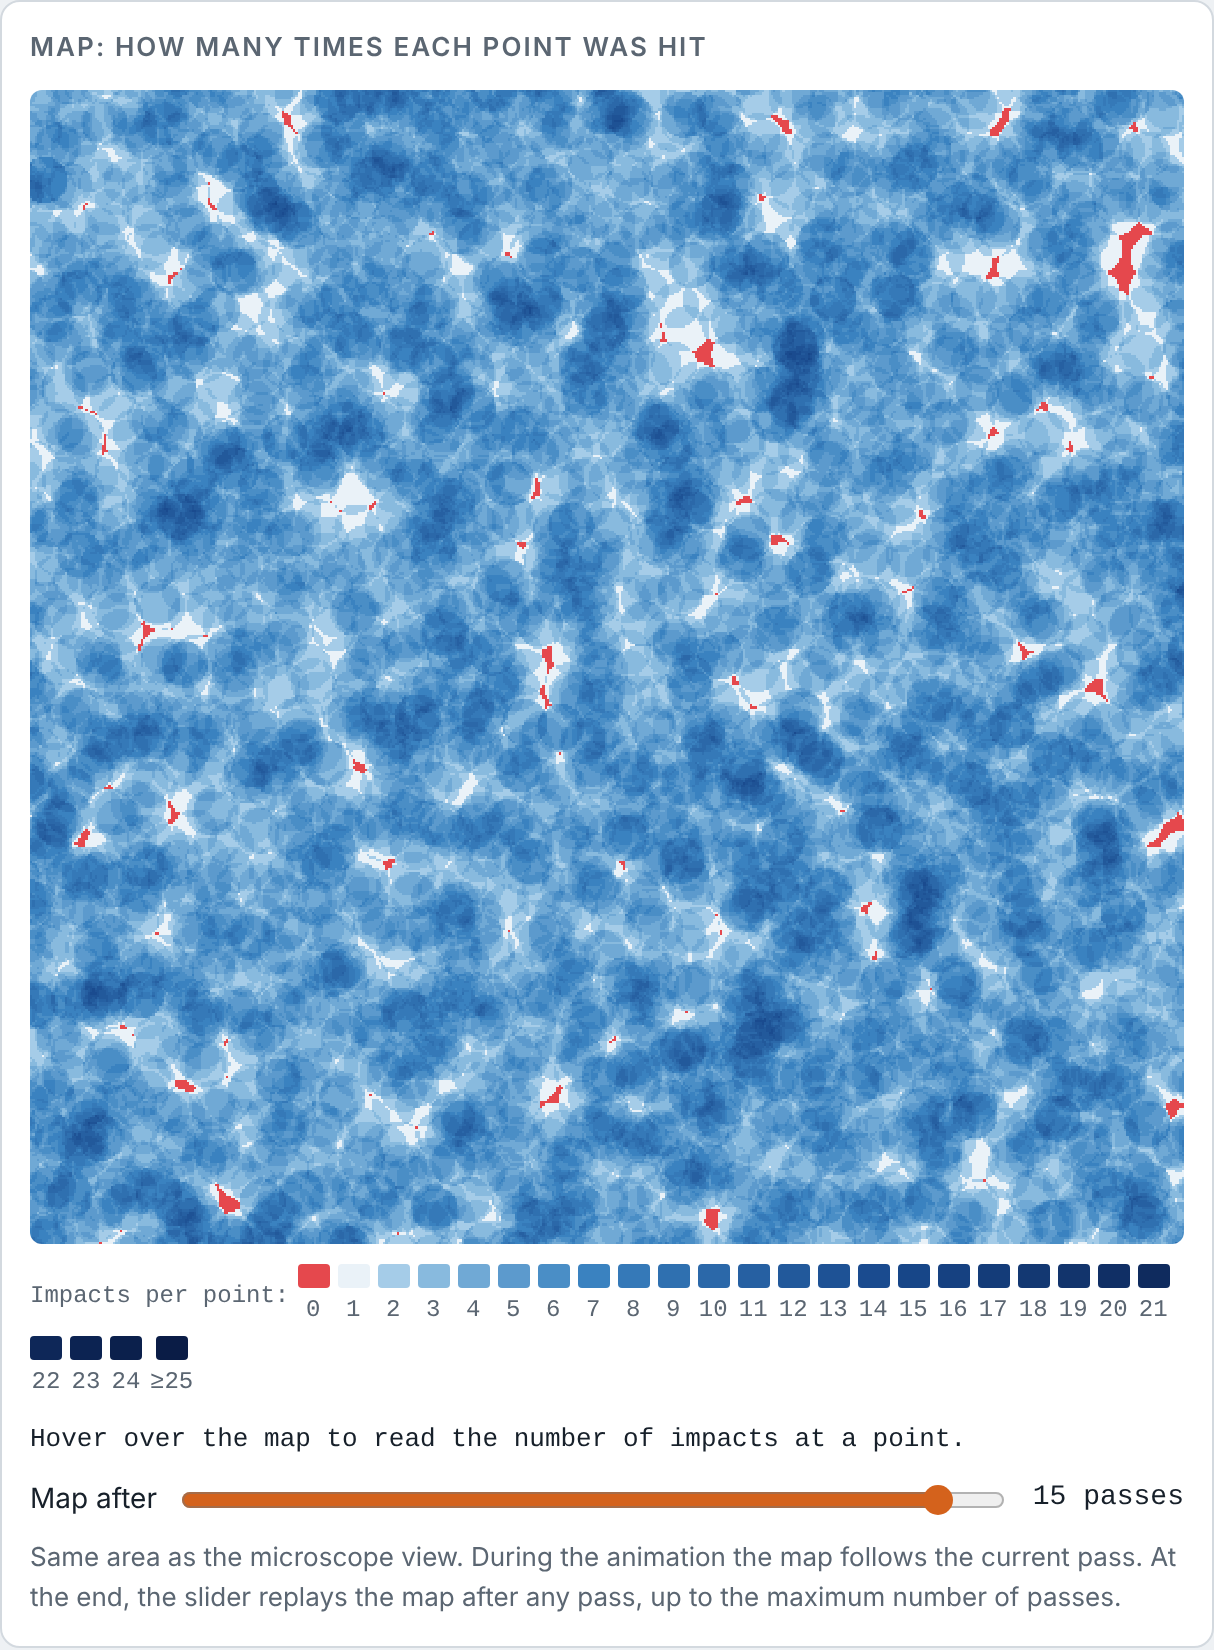
\includegraphics[width=\linewidth]{img/sec2.png}\caption{Hit-count map}\end{subfigure}\hfill
\begin{subfigure}{0.49\linewidth}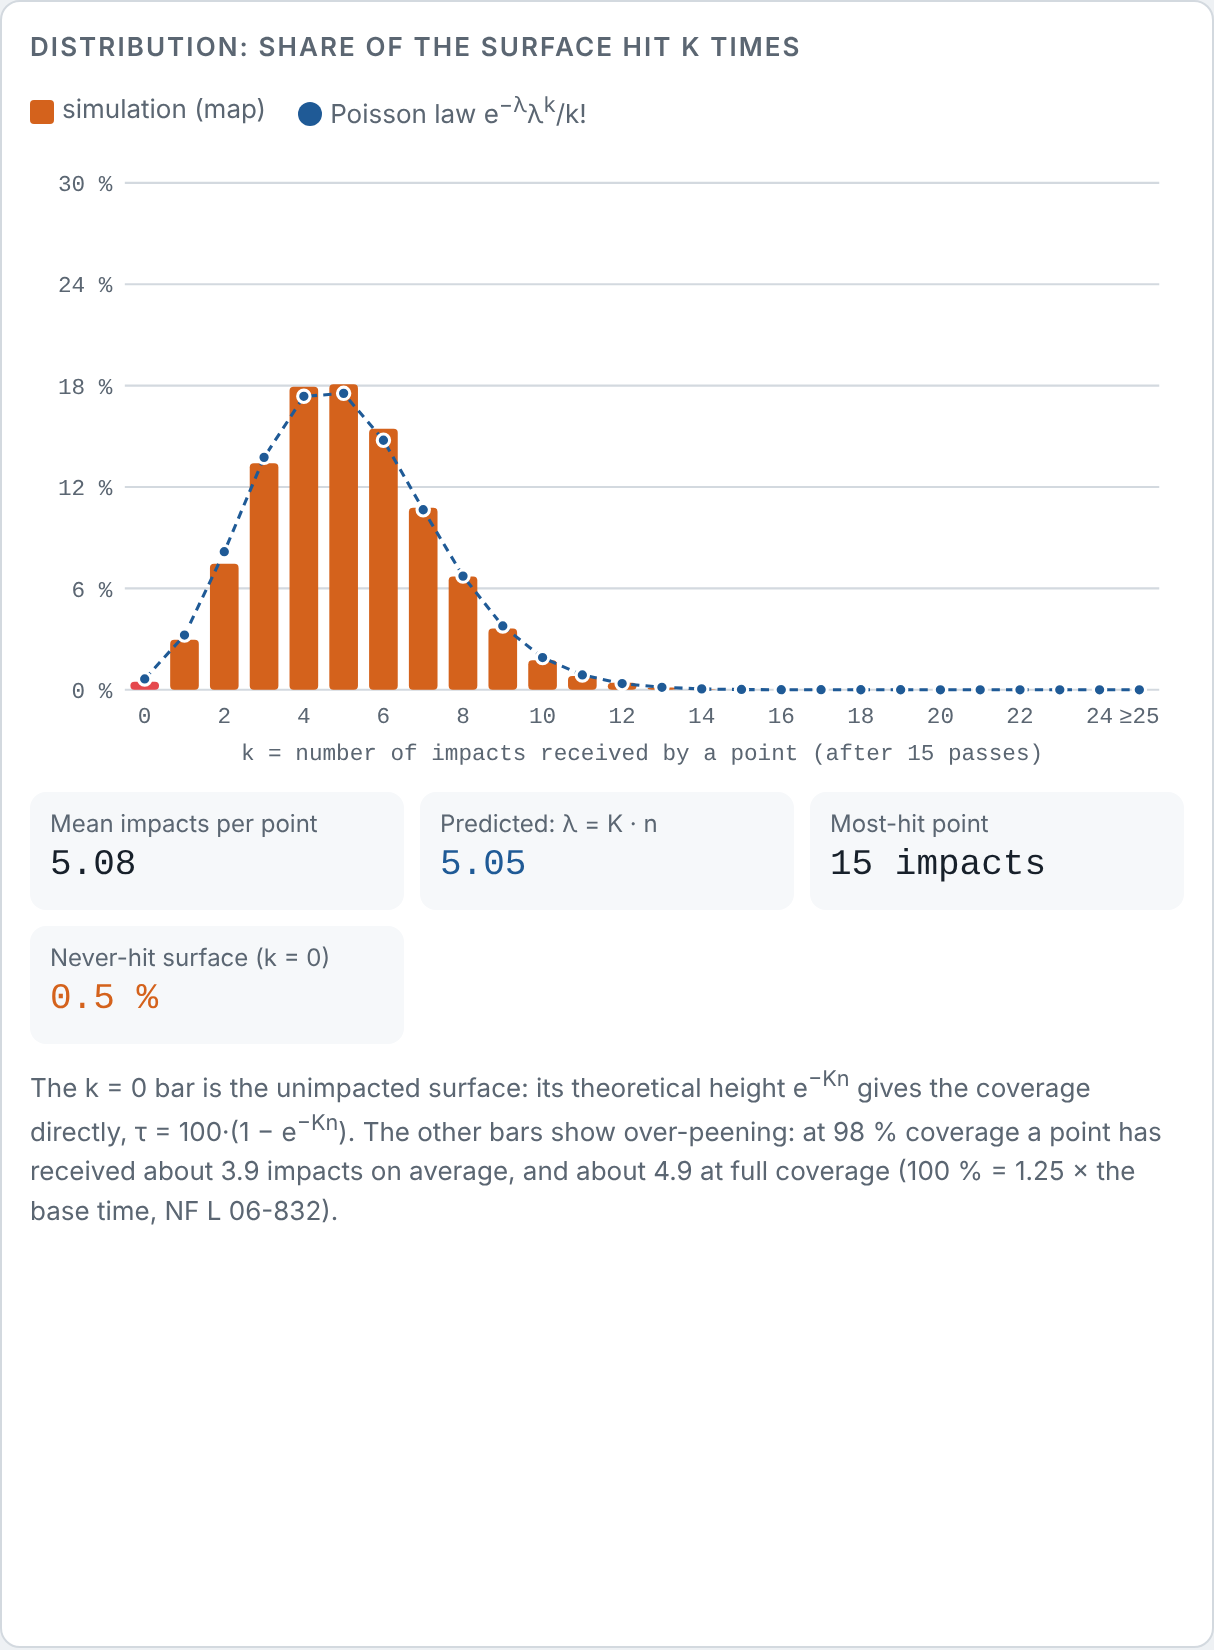
\includegraphics[width=\linewidth]{img/sec3.png}\caption{Distribution of hits}\end{subfigure}
\caption{After 15 passes: almost every point is hit, between 0 and 16 times; the bars follow the Poisson law.}
\end{figure}

\section{Every parameter}\label{sec:params}

\begin{longtable}{@{}p{3.4cm}p{1.55cm}p{2.0cm}p{1.5cm}p{4.9cm}@{}}
\toprule
\textbf{Parameter} & \textbf{Unit} & \textbf{Range} & \textbf{Default} & \textbf{Effect}\\ \midrule\endhead
Media flow rate $\dot m$ & kg/min & 0.1 -- 6 & 1.5 & $K\propto\dot m$: more shots per second.\\
Media density $\rho$ & g/cm³ & 1 -- 8 & 2.2 & $K\propto1/\rho$: heavier shots, fewer of them for the same flow (steel $\approx7.8$, glass $\approx2.5$, ceramic $\approx3.8$).\\
Mass median diameter $D_{50}$ & µm & 30 -- 1000 & 150 & At fixed dent radius, $K\propto1/D_{50}^3$: bigger shots are heavier, so fewer are thrown per second.\\
Size spread $\sigma$ & -- & 0 -- 0.6 & 0 & Log-normal spread; 0 = identical shots. Changes $D_{32}$ and slightly $K$.\\
Jet size $\dX$ & mm & 5 -- 60 & 20 & $K\propto1/\dX$: the same shots spread over a wider band.\\
Traverse speed $V$ & mm/s & 20 -- 1500 & 300 & $K\propto1/V$: a point stays less time under the jet.\\
Dent radius $r$ (for $D=D_{50}$) & µm & 2 -- 100 & 10 & $K\propto r^2$. Measure it on a test coupon; it depends on velocity, material and shot.\\
Number of passes simulated & -- & 1 -- 40 & 15 & Length of the simulation.\\
Specified coverage $C$ & \% & 50 -- 500 & 100 & Specified coverage used for the number of passes and the time (Section~\ref{sec:above}); does not restart the simulation.\\
Full coverage (100\,\%) & -- & 2 choices & 1.25 × base & Whether 100\,\% is 1.25 times the base time (NF~L~06-832) or the base time itself.\\
\bottomrule
\end{longtable}
\noindent Changing a physical parameter restarts the simulation; \ui{Reset to reference values} restores the Excel values.

\section{Coverage above 100\,\% (NF~L~06-832)}\label{sec:above}

Coverage measured as a dented area cannot exceed 100\,\%. Specifications such as ``200\,\% coverage'' refer to \emph{time}. NF~L~06-832 defines:
\begin{itemize}[nosep]
\item the \textbf{base time} $t_b$: the peening time needed to reach 98\,\% coverage (checked visually);
\item \textbf{full coverage, 100\,\%}: $1.25\,t_b$, because 100\,\% cannot be measured;
\item a coverage of \textbf{$C$\,\%}: $\frac{C}{100}\times1.25\,t_b$; 200\,\% is twice the time of full coverage.
\end{itemize}
In the Poisson model time and mean impacts per point are proportional, so these times translate into numbers of impacts and dented areas:

\begin{center}
\begin{tabular}{@{}lccc@{}}
\toprule
Specification & Time & Mean impacts per point $\lambda$ & Dented area\\ \midrule
base time & $t_b$ & $\ln 50=3.91$ & 98\,\%\\
100\,\% & $1.25\,t_b$ & $4.89$ & 99.25\,\%\\
200\,\% & $2.5\,t_b$ & $9.78$ & 99.994\,\%\\
300\,\% & $3.75\,t_b$ & $14.7$ & $\approx100$\,\%\\ \bottomrule
\end{tabular}
\end{center}

\paragraph{The readout \ui{Coverage (NF L 06-832)}.} Coverage is the dented area divided by the total area as long as it can be measured, i.e.\ up to 98\,\%. Beyond, NF~L~06-832 counts time. The page combines both in one value, $C(t)$, continuous and increasing:
\begin{equation}
C(t)=\begin{cases}
\text{dented area (\%)} & t\le t_b\quad(\text{reaches }98\,\%\text{ at }t_b)\\[2pt]
98+2\,\dfrac{t/t_b-1}{0.25} & t_b<t\le1.25\,t_b\quad(98\to100\,\%)\\[6pt]
100\,\dfrac{t}{1.25\,t_b} & t>1.25\,t_b
\end{cases}
\end{equation}
With the option \ui{Full coverage (100\,\%) = base time}, the middle interval disappears: $C=100\,t/t_b$ after the base time. The number of passes (or the time) for a specified coverage $C$ is the inverse of this function: below 98\,\% it comes from the dented area, above 100\,\% it is $\frac{C}{100}\times1.25\,t_b$.

\begin{center}\small
\begin{tabular}{@{}lccccccc@{}}
\toprule
Passes $n$ (reference case, $K=0.337$) & 1 & 3 & 6 & 11.6 ($t_b$) & 13.0 & 14.5 & 29.0\\ \midrule
Dented area (\%) & 28.6 & 63.6 & 86.8 & 98.0 & 98.8 & 99.25 & 99.99\\
Coverage (NF L 06-832) (\%) & 28.6 & 63.6 & 86.8 & 98 & 99 & 100 & 200\\ \bottomrule
\end{tabular}
\end{center}

\paragraph{Local coverage of a point.} On the flat-part and cylinder simulators the same rule is applied to each point, with time replaced by the number of impacts it has received (proportional to time on an even treatment): $C(x,y)=1-e^{-\lambda}$ up to $\lambda=\ln50=3.91$ (98\,\%), then 98 to 100\,\% up to $\lambda=1.25\ln50=4.89$, and $100\,\lambda/4.89$ above. The hover readout gives it, and the map can show it (\ui{Map shows: coverage NF L 06-832}).


\noindent The page gives the number of \ui{Passes for C} ($=\frac{C}{100}\times1.25\,n_{98}$ above 100\,\%). With the option \ui{Full coverage (100\,\%) = base time}, the factor 1.25 is dropped: 100\,\% then means 98\,\% dented and $\lambda=3.91$. The model describes how the surface gets covered; it does not describe what happens physically beyond full coverage (saturation of residual stresses, roughness, over-peening).

\section{Things to try}

\begin{center}
\begin{tabular}{@{}lccccl@{}}
\toprule
Change from the reference & $K$ & $n_{98}$ & $n_{100}$ & Comment\\ \midrule
none (reference) & 0.337 & 11.6 & 14.5 & Excel model\\
$\sigma=0.3$ & 0.352 & 11.1 & 13.9 & $D_{32}=\SI{143}{\micro m}$\\
$V=\SI{600}{mm/s}$ & 0.168 & 23.2 & 29.0 & twice as many passes\\
$\dX=\SI{40}{mm}$ & 0.168 & 23.2 & 29.0 & same effect as doubling $V$\\
$r=\SI{20}{\micro m}$ & 1.347 & 2.9 & 3.6 & $K\propto r^2$: four times faster\\
$\dot m=\SI{3}{kg/min}$ & 0.673 & 5.8 & 7.3 & $K\propto\dot m$\\ \bottomrule
\end{tabular}
\end{center}

\begin{trybox}
\begin{itemize}[nosep,leftmargin=*]
\item Tick \ui{Show unimpacted surface} and play pass by pass with \ui{+1 pass}: the last red spots disappear slowly, which is the exponential law in action.
\item Set 40 passes and look at the histogram: it widens and moves to the right; at 200\,\% coverage ($\approx$ 29 passes) most points receive between about 4 and 16 impacts.
\item Run the same settings several times with \ui{Restart}: the measured points scatter around the blue curve by about one percent.
\item Double $V$ and halve $\dX$: $K$ does not change, because only the product $V\dX$ matters.
\end{itemize}
\end{trybox}

\section{Assumptions and limits}
Uniform jet across its width; every point crosses the jet once per pass; shots land at random, independently; flat surface and normal incidence; dent radius proportional to the shot diameter and independent of the local state of the surface; no rebound, no shot breakage. The model predicts how the surface gets covered, not residual stresses or roughness. It does not replace coverage verification according to the applicable standards (NF~L~06-832, SAE~J2277).

\appendix
\section{Symbols}
\begin{tabular}{@{}ll@{\qquad}ll@{}}
$\tau$ & coverage (dented area, \%) & $K$ & dented area per pass, overlaps counted\\
$n$ & number of passes & $\lambda$ & mean impacts per point\\
$\dot m$ & media flow rate & $\dot N$ & shots per second\\
$\rho$ & media density & $m_p$ & mean shot mass\\
$D_{50}$ & mass median diameter & $D_{32}$ & Sauter diameter $\E[D^3]/\E[D^2]$\\
$\sigma$ & log-normal spread & $c$ & ratio dent radius / shot diameter\\
$r$ & dent radius & $R$ & impacts per mm² per pass\\
$V$ & traverse speed & $\dX$ & jet size\\
$t_b$ & base time (98\,\%) & $C$ & specified coverage\\
\end{tabular}

\vfill
\noindent\small Code: MIT licence. Documentation: CC BY 4.0. Related tools: Extended Shot Peening Coverage Simulator (flat part, raster paths), Cylinder Shot Peening Coverage Simulator, Piezopeening Coverage Simulator: \url{https://rkubler.github.io/shotpeening/}.
\end{document}
